% Densidad aparente relativa a la de 1 kPa, rho/rho_0 = (sigma/1 kPa)^c, con
% los exponentes de Lanzerstorfer (2020, Tabla 2): harina de trigo W 480 (F2),
% azúcar impalpable (S1), azúcar cristal (S3) y sal de mesa (I3).
% Escala: 0,4 cm por kPa y 0,12 cm por punto porcentual desde 90 %.
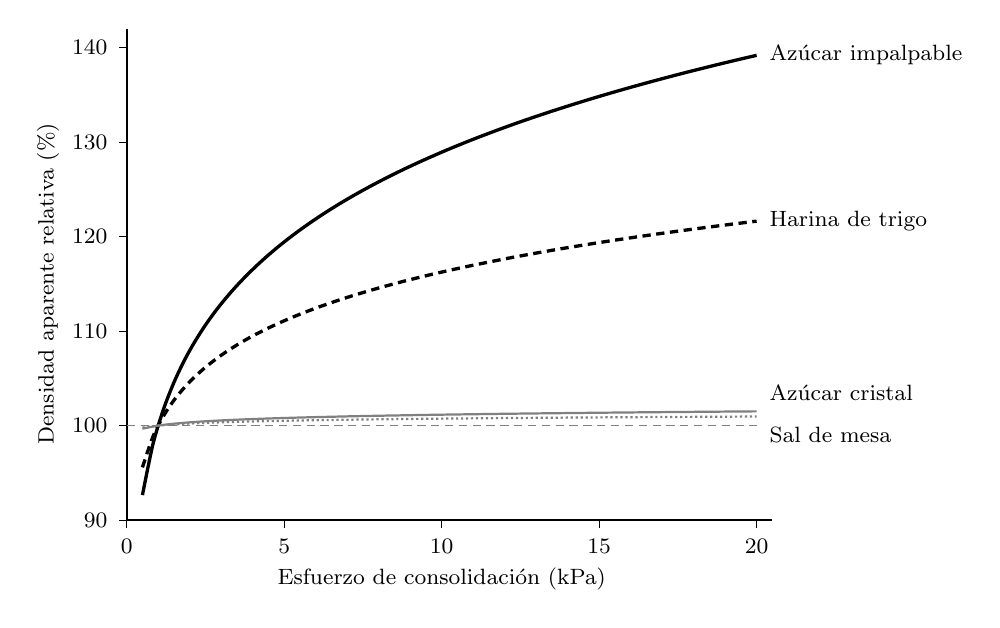
\begin{tikzpicture}[font=\small, nota/.style={font=\footnotesize, align=left}]
\def\sx{0.4}
\def\sy{0.12}

% Ejes
\draw[thick] (0,0) -- ({\sx*20.5},0);
\draw[thick] (0,0) -- (0,{\sy*52});
\foreach \x in {0,5,10,15,20}{
    \draw ({\sx*\x},0) -- ({\sx*\x},-0.1);
    \node[nota, anchor=north] at ({\sx*\x},-0.12) {\x};
}
\foreach \y in {90,100,110,120,130,140}{
    \draw (0,{\sy*(\y-90)}) -- (-0.1,{\sy*(\y-90)});
    \node[nota, anchor=east] at (-0.12,{\sy*(\y-90)}) {\y};
}
\node[font=\footnotesize] at ({\sx*10},-0.75) {Esfuerzo de consolidación (kPa)};
\node[font=\footnotesize, rotate=90] at (-1.0,{\sy*25}) {Densidad aparente relativa (\%)};
\draw[densely dashed, gray] (0,{\sy*10}) -- ({\sx*20},{\sy*10});

% Curvas
\draw[very thick] plot[domain=0.5:20, samples=60, smooth]
    ({\sx*\x}, {\sy*(100*pow(\x,0.1104)-90)});
\draw[very thick, densely dashed] plot[domain=0.5:20, samples=60, smooth]
    ({\sx*\x}, {\sy*(100*pow(\x,0.0654)-90)});
\draw[thick, gray] plot[domain=0.5:20, samples=40, smooth]
    ({\sx*\x}, {\sy*(100*pow(\x,0.0050)-90)});
\draw[thick, gray, densely dotted] plot[domain=0.5:20, samples=40, smooth]
    ({\sx*\x}, {\sy*(100*pow(\x,0.0032)-90)});

% Rótulos al final de cada curva
\node[nota, anchor=west] at ({\sx*20.1},{\sy*(139.2-90)}) {Azúcar impalpable};
\node[nota, anchor=west] at ({\sx*20.1},{\sy*(121.7-90)}) {Harina de trigo};
\node[nota, anchor=west] at ({\sx*20.1},{\sy*(103.5-90)}) {Azúcar cristal};
\node[nota, anchor=west] at ({\sx*20.1},{\sy*(99.0-90)}) {Sal de mesa};
\end{tikzpicture}
